\documentclass[]{standalone}

\usepackage{pgf}
\usepackage{tikz}
\usetikzlibrary{arrows,automata,matrix}
\usepackage[latin1]{inputenc}
\begin{document}
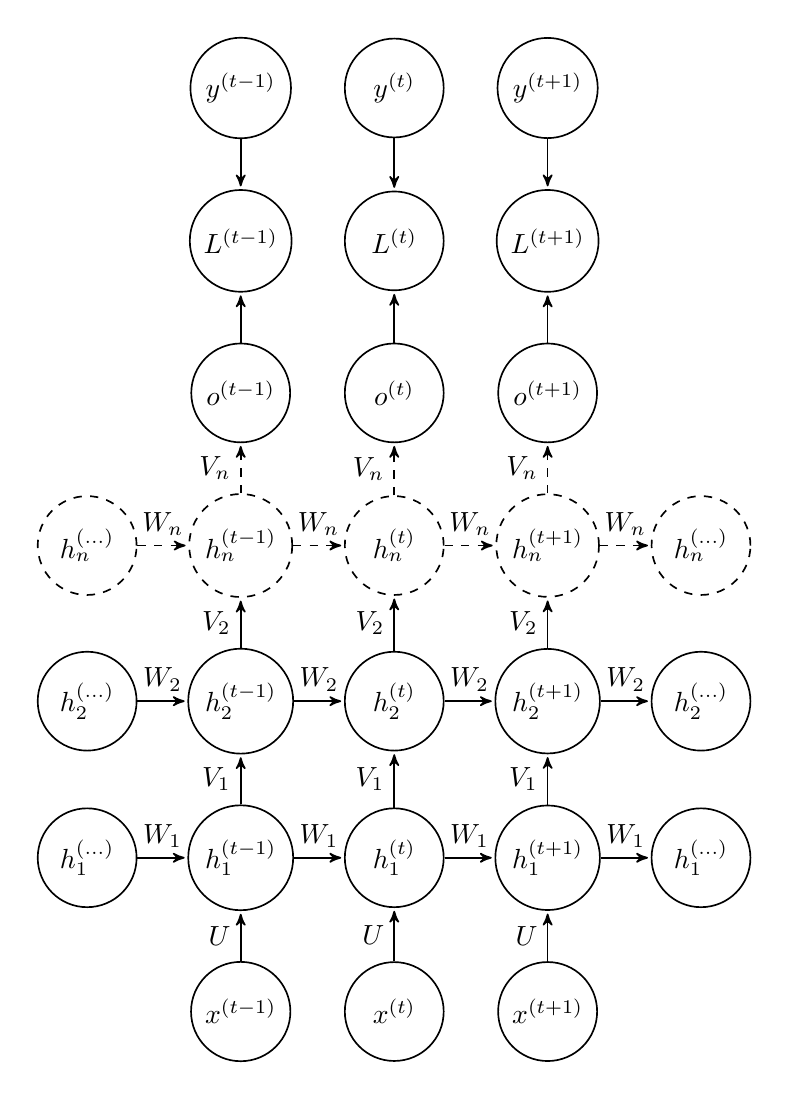
\begin{tikzpicture}[->,>=stealth'
	,shorten >=1pt
	,auto
	,node distance=2.8cm,
              semithick]
  \tikzstyle{every state}=[minimum size={10pt+width("$x^{(t-1)}$")}]

  \matrix (m) [matrix of nodes
  ,row sep=.25in,column sep=.25in] {
    % 3 ys
    &
    \node[state](ytm1) {$y^{(t-1)}$}; &
    \node[state](yt) {$y^{(t)}$};    &
    \node[state](ytp1) {$y^{(t+1)}$}; 
    \\
    % 3 Ls
    &
    \node[state](Ltm1) {$L^{(t-1)}$}; &
    \node[state](Lt) {$L^{(t)}$}; &
    \node[state](Ltp1) {$L^{(t+1)}$};
    \\
    % 3 os
    &
    \node[state](otm1) {$o^{(t-1)}$}; &
    \node[state](ot) {$o^{(t)}$}; &
    \node[state](otp1) {$o^{(t+1)}$};
    \\
    % 5 hns
    \node[state,dashed](hndm) {$h_n^{(\ldots)}$}; &
    \node[state,dashed](hntm1) {$h_n^{(t-1)}$}; &
    \node[state,dashed](hnt) {$h_n^{(t)}$}; &
    \node[state,dashed](hntp1) {$h_n^{(t+1)}$}; &
    \node[state,dashed](hndp) {$h_n^{(\ldots)}$};
    \\
    % 5 h2s
    \node[state](h2dm) {$h_2^{(\ldots)}$}; &
    \node[state](h2tm1) {$h_2^{(t-1)}$}; &
    \node[state](h2t) {$h_2^{(t)}$}; &
    \node[state](h2tp1) {$h_2^{(t+1)}$}; &
    \node[state](h2dp) {$h_2^{(\ldots)}$};
    \\
    % 5 h1s
    \node[state](h1dm) {$h_1^{(\ldots)}$}; &
    \node[state](h1tm1) {$h_1^{(t-1)}$}; &
    \node[state](h1t) {$h_1^{(t)}$}; &
    \node[state](h1tp1) {$h_1^{(t+1)}$}; &
    \node[state](h1dp) {$h_1^{(\ldots)}$}; 
    \\
    % 3 xs
    &
    \node[state](xtm1) {$x^{(t-1)}$}; &
    \node[state](xt) {$x^{(t)}$};    &
    \node[state](xtp1) {$x^{(t+1)}$};
    \\
  };
  % left to right, top to bottom.
  % each layer outgoing and within itself arrows
  % minus ... 
  \path [dashed] (hndm)  edge  node {$W_n$} (hntm1);
  \path [      ] (h2dm)  edge  node {$W_2$} (h2tm1);
  \path [      ] (h1dm)  edge  node {$W_1$} (h1tm1);
  % t-1
  \path [      ] (ytm1)  edge  node {     } (Ltm1);
  \path [      ] (otm1)  edge  node {     } (Ltm1);
  \path [dashed] (hntm1) edge  node {$V_n$} (otm1);
  \path [      ] (h2tm1) edge  node {$V_2$} (hntm1);
  \path [      ] (h1tm1) edge  node {$V_1$} (h2tm1);
  \path [      ] (xtm1)  edge  node {$U$}   (h1tm1);
  \path [dashed] (hntm1) edge  node {$W_n$} (hnt);
  \path [      ] (h2tm1) edge  node {$W_2$} (h2t);
  \path [      ] (h1tm1) edge  node {$W_1$} (h1t);
  % t
  \path [      ] (yt)    edge  node {     } (Lt);
  \path [      ] (ot)    edge  node {     } (Lt);
  \path [dashed] (hnt)   edge  node {$V_n$} (ot);
  \path [      ] (h2t)   edge  node {$V_2$} (hnt);
  \path [      ] (h1t)   edge  node {$V_1$} (h2t);
  \path [      ] (xt)    edge  node {$U$}   (h1t);
  \path [dashed] (hnt)   edge  node {$W_n$} (hntp1);
  \path [      ] (h2t)   edge  node {$W_2$} (h2tp1);
  \path [      ] (h1t)   edge  node {$W_1$} (h1tp1);
  % t+1
  \path [      ] (ytp1)  edge  node {     } (Ltp1);
  \path [      ] (otp1)  edge  node {     } (Ltp1);
  \path [dashed] (hntp1) edge  node {$V_n$} (otp1);
  \path [      ] (h2tp1) edge  node {$V_2$} (hntp1);
  \path [      ] (h1tp1) edge  node {$V_1$} (h2tp1);
  \path [      ] (xtp1)  edge  node {$U$}   (h1tp1);
  \path [dashed] (hntp1) edge  node {$W_n$} (hndp);
  \path [      ] (h2tp1) edge  node {$W_2$} (h2dp);
  \path [      ] (h1tp1) edge  node {$W_1$} (h1dp);

  
\end{tikzpicture}

\end{document}